\documentclass[1p]{elsarticle_modified}
%\bibliographystyle{elsarticle-num}

%\usepackage[colorlinks]{hyperref}
%\usepackage{abbrmath_seonhwa} %\Abb, \Ascr, \Acal ,\Abf, \Afrak
\usepackage{amsfonts}
\usepackage{amssymb}
\usepackage{amsmath}
\usepackage{amsthm}
\usepackage{scalefnt}
\usepackage{amsbsy}
\usepackage{kotex}
\usepackage{caption}
\usepackage{subfig}
\usepackage{color}
\usepackage{graphicx}
\usepackage{xcolor} %% white, black, red, green, blue, cyan, magenta, yellow
\usepackage{float}
\usepackage{setspace}
\usepackage{hyperref}

\usepackage{tikz}
\usetikzlibrary{arrows}

\usepackage{multirow}
\usepackage{array} % fixed length table
\usepackage{hhline}

%%%%%%%%%%%%%%%%%%%%%
\makeatletter
\renewcommand*\env@matrix[1][\arraystretch]{%
	\edef\arraystretch{#1}%
	\hskip -\arraycolsep
	\let\@ifnextchar\new@ifnextchar
	\array{*\c@MaxMatrixCols c}}
\makeatother %https://tex.stackexchange.com/questions/14071/how-can-i-increase-the-line-spacing-in-a-matrix
%%%%%%%%%%%%%%%

\usepackage[normalem]{ulem}

\newcommand{\msout}[1]{\ifmmode\text{\sout{\ensuremath{#1}}}\else\sout{#1}\fi}
%SOURCE: \msout is \stkout macro in https://tex.stackexchange.com/questions/20609/strikeout-in-math-mode

\newcommand{\cancel}[1]{
	\ifmmode
	{\color{red}\msout{#1}}
	\else
	{\color{red}\sout{#1}}
	\fi
}

\newcommand{\add}[1]{
	{\color{blue}\uwave{#1}}
}

\newcommand{\replace}[2]{
	\ifmmode
	{\color{red}\msout{#1}}{\color{blue}\uwave{#2}}
	\else
	{\color{red}\sout{#1}}{\color{blue}\uwave{#2}}
	\fi
}

\newcommand{\Sol}{\mathcal{S}} %segment
\newcommand{\D}{D} %diagram
\newcommand{\A}{\mathcal{A}} %arc


%%%%%%%%%%%%%%%%%%%%%%%%%%%%%5 test

\def\sl{\operatorname{\textup{SL}}(2,\Cbb)}
\def\psl{\operatorname{\textup{PSL}}(2,\Cbb)}
\def\quan{\mkern 1mu \triangleright \mkern 1mu}

\theoremstyle{definition}
\newtheorem{thm}{Theorem}[section]
\newtheorem{prop}[thm]{Proposition}
\newtheorem{lem}[thm]{Lemma}
\newtheorem{ques}[thm]{Question}
\newtheorem{cor}[thm]{Corollary}
\newtheorem{defn}[thm]{Definition}
\newtheorem{exam}[thm]{Example}
\newtheorem{rmk}[thm]{Remark}
\newtheorem{alg}[thm]{Algorithm}

\newcommand{\I}{\sqrt{-1}}
\begin{document}

%\begin{frontmatter}
%
%\title{Boundary parabolic representations of knots up to 8 crossings}
%
%%% Group authors per affiliation:
%\author{Yunhi Cho} 
%\address{Department of Mathematics, University of Seoul, Seoul, Korea}
%\ead{yhcho@uos.ac.kr}
%
%
%\author{Seonhwa Kim} %\fnref{s_kim}}
%\address{Center for Geometry and Physics, Institute for Basic Science, Pohang, 37673, Korea}
%\ead{ryeona17@ibs.re.kr}
%
%\author{Hyuk Kim}
%\address{Department of Mathematical Sciences, Seoul National University, Seoul 08826, Korea}
%\ead{hyukkim@snu.ac.kr}
%
%\author{Seokbeom Yoon}
%\address{Department of Mathematical Sciences, Seoul National University, Seoul, 08826,  Korea}
%\ead{sbyoon15@snu.ac.kr}
%
%\begin{abstract}
%We find all boundary parabolic representation of knots up to 8 crossings.
%
%\end{abstract}
%\begin{keyword}
%    \MSC[2010] 57M25 
%\end{keyword}
%
%\end{frontmatter}

%\linenumbers
%\tableofcontents
%
\newcommand\colored[1]{\textcolor{white}{\rule[-0.35ex]{0.8em}{1.4ex}}\kern-0.8em\color{red} #1}%
%\newcommand\colored[1]{\textcolor{white}{ #1}\kern-2.17ex	\textcolor{white}{ #1}\kern-1.81ex	\textcolor{white}{ #1}\kern-2.15ex\color{red}#1	}

{\Large $\underline{11a_{279}~(K11a_{279})}$}

\setlength{\tabcolsep}{10pt}
\renewcommand{\arraystretch}{1.6}
\vspace{1cm}\begin{tabular}{m{100pt}>{\centering\arraybackslash}m{274pt}}
\multirow{5}{120pt}{
	\centering
	\includegraphics[width=112pt]{../../../GIT/diagram.site/Diagrams/png/528_11a_279.png}\\
\ \ \ A knot diagram\footnotemark}&
\allowdisplaybreaks
\textbf{Linearized knot diagam} \\
\cline{2-2}
 &
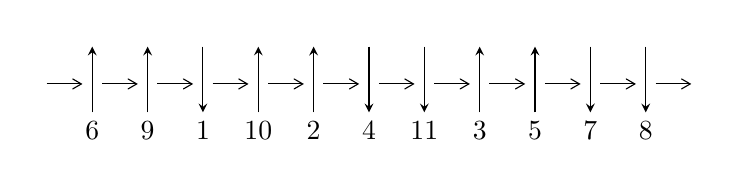
\begin{tikzpicture}[x=20pt, y=17pt]
	% nodes
	\node (C0) at (0, 0) {};
	\node (C1) at (1, 0) {};
	\node (C1U) at (1, +1) {};
	\node (C1D) at (1, -1) {6};

	\node (C2) at (2, 0) {};
	\node (C2U) at (2, +1) {};
	\node (C2D) at (2, -1) {9};

	\node (C3) at (3, 0) {};
	\node (C3U) at (3, +1) {};
	\node (C3D) at (3, -1) {1};

	\node (C4) at (4, 0) {};
	\node (C4U) at (4, +1) {};
	\node (C4D) at (4, -1) {10};

	\node (C5) at (5, 0) {};
	\node (C5U) at (5, +1) {};
	\node (C5D) at (5, -1) {2};

	\node (C6) at (6, 0) {};
	\node (C6U) at (6, +1) {};
	\node (C6D) at (6, -1) {4};

	\node (C7) at (7, 0) {};
	\node (C7U) at (7, +1) {};
	\node (C7D) at (7, -1) {11};

	\node (C8) at (8, 0) {};
	\node (C8U) at (8, +1) {};
	\node (C8D) at (8, -1) {3};

	\node (C9) at (9, 0) {};
	\node (C9U) at (9, +1) {};
	\node (C9D) at (9, -1) {5};

	\node (C10) at (10, 0) {};
	\node (C10U) at (10, +1) {};
	\node (C10D) at (10, -1) {7};

	\node (C11) at (11, 0) {};
	\node (C11U) at (11, +1) {};
	\node (C11D) at (11, -1) {8};
	\node (C12) at (12, 0) {};

	% arrows
	\draw[->,>={angle 60}]
	(C0) edge (C1) (C1) edge (C2) (C2) edge (C3) (C3) edge (C4) (C4) edge (C5) (C5) edge (C6) (C6) edge (C7) (C7) edge (C8) (C8) edge (C9) (C9) edge (C10) (C10) edge (C11) (C11) edge (C12) ;	\draw[->,>=stealth]
	(C1D) edge (C1U) (C2D) edge (C2U) (C3U) edge (C3D) (C4D) edge (C4U) (C5D) edge (C5U) (C6U) edge (C6D) (C7U) edge (C7D) (C8D) edge (C8U) (C9D) edge (C9U) (C10U) edge (C10D) (C11U) edge (C11D) ;
	\end{tikzpicture} \\
\hhline{~~} \\& 
\textbf{Solving Sequence} \\ \cline{2-2} 
 &
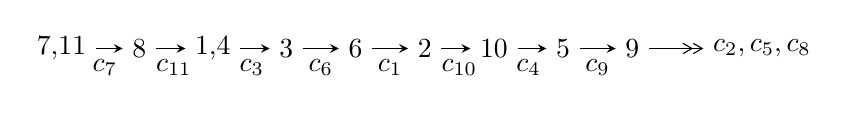
\begin{tikzpicture}[x=25pt, y=7pt]
	% node
	\node (A0) at (-1/8, 0) {7,11};
	\node (A1) at (1, 0) {8};
	\node (A2) at (33/16, 0) {1,4};
	\node (A3) at (25/8, 0) {3};
	\node (A4) at (33/8, 0) {6};
	\node (A5) at (41/8, 0) {2};
	\node (A6) at (49/8, 0) {10};
	\node (A7) at (57/8, 0) {5};
	\node (A8) at (65/8, 0) {9};
	\node (C1) at (1/2, -1) {$c_{7}$};
	\node (C2) at (3/2, -1) {$c_{11}$};
	\node (C3) at (21/8, -1) {$c_{3}$};
	\node (C4) at (29/8, -1) {$c_{6}$};
	\node (C5) at (37/8, -1) {$c_{1}$};
	\node (C6) at (45/8, -1) {$c_{10}$};
	\node (C7) at (53/8, -1) {$c_{4}$};
	\node (C8) at (61/8, -1) {$c_{9}$};
	\node (A9) at (10, 0) {$c_{2},c_{5},c_{8}$};

	% edge
	\draw[->,>=stealth]	
	(A0) edge (A1) (A1) edge (A2) (A2) edge (A3) (A3) edge (A4) (A4) edge (A5) (A5) edge (A6) (A6) edge (A7) (A7) edge (A8) ;
	\draw[->>,>={angle 60}]	
	(A8) edge (A9);
\end{tikzpicture} \\ 

\end{tabular} \\

\footnotetext{
The image of knot diagram is generated by the software ``\textbf{Draw programme}" developed by Andrew Bartholomew(\url{http://www.layer8.co.uk/maths/draw/index.htm\#Running-draw}), where we modified some parts for our purpose(\url{https://github.com/CATsTAILs/LinksPainter}).
}\phantom \\ \newline 
\centering \textbf{Ideals for irreducible components\footnotemark of $X_{\text{par}}$} 
 
\begin{align*}
I^u_{1}&=\langle 
-207 u^{22}+1583 u^{21}+\cdots+4 b-1196,\;-703 u^{22}+5325 u^{21}+\cdots+8 a-3908,\\
\phantom{I^u_{1}}&\phantom{= \langle  }u^{23}-9 u^{22}+\cdots-16 u-8\rangle \\
I^u_{2}&=\langle 
-67075021335 a^5 u^5-139677423007 u^5 a^4+\cdots+70899952257 a-101012825507,\\
\phantom{I^u_{2}}&\phantom{= \langle  }a^5 u^5-8 u^5 a^4+\cdots-56 a+146,\;u^6+u^5-3 u^4-2 u^3+2 u^2- u-1\rangle \\
I^u_{3}&=\langle 
u^{13}+u^{12}-6 u^{11}-6 u^{10}+13 u^9+12 u^8-15 u^7-10 u^6+14 u^5+5 u^4-8 u^3- u^2+b+2 u,\\
\phantom{I^u_{3}}&\phantom{= \langle  }u^{11}-6 u^9+13 u^7- u^6-14 u^5+4 u^4+10 u^3-5 u^2+a-3 u+2,\\
\phantom{I^u_{3}}&\phantom{= \langle  }u^{14}+2 u^{13}-6 u^{12}-13 u^{11}+13 u^{10}+31 u^9-15 u^8-36 u^7+15 u^6+26 u^5-11 u^4-12 u^3+3 u^2+2 u+1\rangle \\
\\
\end{align*}
\raggedright * 3 irreducible components of $\dim_{\mathbb{C}}=0$, with total 73 representations.\\
\footnotetext{All coefficients of polynomials are rational numbers. But the coefficients are sometimes approximated in decimal forms when there is not enough margin.}
\newpage
\renewcommand{\arraystretch}{1}
\centering \section*{I. $I^u_{1}= \langle -207 u^{22}+1583 u^{21}+\cdots+4 b-1196,\;-703 u^{22}+5325 u^{21}+\cdots+8 a-3908,\;u^{23}-9 u^{22}+\cdots-16 u-8 \rangle$}
\flushleft \textbf{(i) Arc colorings}\\
\begin{tabular}{m{7pt} m{180pt} m{7pt} m{180pt} }
\flushright $a_{7}=$&$\begin{pmatrix}1\\0\end{pmatrix}$ \\
\flushright $a_{11}=$&$\begin{pmatrix}0\\u\end{pmatrix}$ \\
\flushright $a_{8}=$&$\begin{pmatrix}1\\u^2\end{pmatrix}$ \\
\flushright $a_{1}=$&$\begin{pmatrix}- u\\- u^3+u\end{pmatrix}$ \\
\flushright $a_{4}=$&$\begin{pmatrix}87.8750 u^{22}-665.625 u^{21}+\cdots+1316.50 u+488.500\\\frac{207}{4} u^{22}-\frac{1583}{4} u^{21}+\cdots+\frac{1625}{2} u+299\end{pmatrix}$ \\
\flushright $a_{3}=$&$\begin{pmatrix}17.8750 u^{22}-127.625 u^{21}+\cdots+189.500 u+74.5000\\\frac{23}{4} u^{22}-\frac{107}{4} u^{21}+\cdots-\frac{185}{2} u-23\end{pmatrix}$ \\
\flushright $a_{6}=$&$\begin{pmatrix}-27 u^{22}+202 u^{21}+\cdots-\frac{737}{2} u-\frac{279}{2}\\-\frac{41}{2} u^{22}+155 u^{21}+\cdots-\frac{599}{2} u-112\end{pmatrix}$ \\
\flushright $a_{2}=$&$\begin{pmatrix}-\frac{89}{2} u^{22}+\frac{1365}{4} u^{21}+\cdots-\frac{2899}{4} u-264\\-\frac{127}{4} u^{22}+\frac{973}{4} u^{21}+\cdots-523 u-190\end{pmatrix}$ \\
\flushright $a_{10}=$&$\begin{pmatrix}u\\u\end{pmatrix}$ \\
\flushright $a_{5}=$&$\begin{pmatrix}2.87500 u^{22}-31.6250 u^{21}+\cdots+143.500 u+46.5000\\-\frac{133}{4} u^{22}+\frac{953}{4} u^{21}+\cdots-\frac{721}{2} u-143\end{pmatrix}$ \\
\flushright $a_{9}=$&$\begin{pmatrix}-14 u^{22}+106 u^{21}+\cdots-\frac{403}{2} u-\frac{151}{2}\\-20 u^{22}+\frac{305}{2} u^{21}+\cdots-\frac{599}{2} u-112\end{pmatrix}$\\ \flushright $a_{9}=$&$\begin{pmatrix}-14 u^{22}+106 u^{21}+\cdots-\frac{403}{2} u-\frac{151}{2}\\-20 u^{22}+\frac{305}{2} u^{21}+\cdots-\frac{599}{2} u-112\end{pmatrix}$\\&\end{tabular}
\flushleft \textbf{(ii) Obstruction class $= -1$}\\~\\
\flushleft \textbf{(iii) Cusp Shapes $= 170 u^{22}-1286 u^{21}+3085 u^{20}-847 u^{19}-4606 u^{18}-3555 u^{17}+14615 u^{16}+14163 u^{15}-31843 u^{14}-26814 u^{13}+25733 u^{12}+61934 u^{11}-11560 u^{10}-75044 u^9-12076 u^8+43840 u^7+41946 u^6-26305 u^5-16870 u^4-1708 u^3+3903 u^2+2554 u+954$}\\~\\
\newpage\renewcommand{\arraystretch}{1}
\flushleft \textbf{(iv) u-Polynomials at the component}\newline \\
\begin{tabular}{m{50pt}|m{274pt}}
Crossings & \hspace{64pt}u-Polynomials at each crossing \\
\hline $$\begin{aligned}c_{1},c_{5}\end{aligned}$$&$\begin{aligned}
&u^{23}-14 u^{22}+\cdots+608 u-64
\end{aligned}$\\
\hline $$\begin{aligned}c_{2},c_{4},c_{8}\\c_{9}\end{aligned}$$&$\begin{aligned}
&u^{23}+12 u^{21}+\cdots+2 u+1
\end{aligned}$\\
\hline $$\begin{aligned}c_{3},c_{6}\end{aligned}$$&$\begin{aligned}
&u^{23}-2 u^{22}+\cdots-10 u-1
\end{aligned}$\\
\hline $$\begin{aligned}c_{7},c_{10},c_{11}\end{aligned}$$&$\begin{aligned}
&u^{23}+9 u^{22}+\cdots-16 u+8
\end{aligned}$\\
\hline
\end{tabular}\\~\\
\newpage\renewcommand{\arraystretch}{1}
\flushleft \textbf{(v) Riley Polynomials at the component}\newline \\
\begin{tabular}{m{50pt}|m{274pt}}
Crossings & \hspace{64pt}Riley Polynomials at each crossing \\
\hline $$\begin{aligned}c_{1},c_{5}\end{aligned}$$&$\begin{aligned}
&y^{23}+12 y^{22}+\cdots-3072 y-4096
\end{aligned}$\\
\hline $$\begin{aligned}c_{2},c_{4},c_{8}\\c_{9}\end{aligned}$$&$\begin{aligned}
&y^{23}+24 y^{22}+\cdots+2 y-1
\end{aligned}$\\
\hline $$\begin{aligned}c_{3},c_{6}\end{aligned}$$&$\begin{aligned}
&y^{23}-16 y^{22}+\cdots+58 y-1
\end{aligned}$\\
\hline $$\begin{aligned}c_{7},c_{10},c_{11}\end{aligned}$$&$\begin{aligned}
&y^{23}-23 y^{22}+\cdots-32 y-64
\end{aligned}$\\
\hline
\end{tabular}\\~\\
\newpage\flushleft \textbf{(vi) Complex Volumes and Cusp Shapes}
$$\begin{array}{c|c|c}  
\text{Solutions to }I^u_{1}& \I (\text{vol} + \sqrt{-1}CS) & \text{Cusp shape}\\
 \hline 
\begin{aligned}
u &= \phantom{-}0.967745 + 0.381665 I \\
a &= \phantom{-}0.201884 + 0.414286 I \\
b &= -0.183628 - 0.001198 I\end{aligned}
 & -1.61771 - 1.40406 I & -4.39049 - 3.86592 I \\ \hline\begin{aligned}
u &= \phantom{-}0.967745 - 0.381665 I \\
a &= \phantom{-}0.201884 - 0.414286 I \\
b &= -0.183628 + 0.001198 I\end{aligned}
 & -1.61771 + 1.40406 I & -4.39049 + 3.86592 I \\ \hline\begin{aligned}
u &= -0.698852 + 0.821638 I \\
a &= \phantom{-}0.477872 + 0.534934 I \\
b &= \phantom{-}1.29859 - 0.66746 I\end{aligned}
 & -10.9998 + 10.3816 I & -5.93991 - 6.82804 I \\ \hline\begin{aligned}
u &= -0.698852 - 0.821638 I \\
a &= \phantom{-}0.477872 - 0.534934 I \\
b &= \phantom{-}1.29859 + 0.66746 I\end{aligned}
 & -10.9998 - 10.3816 I & -5.93991 + 6.82804 I \\ \hline\begin{aligned}
u &= -0.497254 + 0.985536 I \\
a &= -0.155208 + 0.547360 I \\
b &= \phantom{-}1.111120 + 0.180964 I\end{aligned}
 & -10.27160 - 4.44360 I & -7.21311 + 2.51122 I \\ \hline\begin{aligned}
u &= -0.497254 - 0.985536 I \\
a &= -0.155208 - 0.547360 I \\
b &= \phantom{-}1.111120 - 0.180964 I\end{aligned}
 & -10.27160 + 4.44360 I & -7.21311 - 2.51122 I \\ \hline\begin{aligned}
u &= -1.143500 + 0.155903 I \\
a &= -0.153289 + 0.400091 I \\
b &= -0.166969 + 1.049480 I\end{aligned}
 & -2.11154 + 2.89602 I & -5.87366 - 5.40163 I \\ \hline\begin{aligned}
u &= -1.143500 - 0.155903 I \\
a &= -0.153289 - 0.400091 I \\
b &= -0.166969 - 1.049480 I\end{aligned}
 & -2.11154 - 2.89602 I & -5.87366 + 5.40163 I \\ \hline\begin{aligned}
u &= -0.712264 + 0.994425 I \\
a &= -0.160694 - 0.410443 I \\
b &= -1.026660 + 0.292744 I\end{aligned}
 & -5.31535 + 3.36271 I & -7.37506 - 4.35567 I \\ \hline\begin{aligned}
u &= -0.712264 - 0.994425 I \\
a &= -0.160694 + 0.410443 I \\
b &= -1.026660 - 0.292744 I\end{aligned}
 & -5.31535 - 3.36271 I & -7.37506 + 4.35567 I\\
 \hline 
 \end{array}$$\newpage$$\begin{array}{c|c|c}  
\text{Solutions to }I^u_{1}& \I (\text{vol} + \sqrt{-1}CS) & \text{Cusp shape}\\
 \hline 
\begin{aligned}
u &= \phantom{-}1.42821\phantom{ +0.000000I} \\
a &= \phantom{-}1.51970\phantom{ +0.000000I} \\
b &= \phantom{-}0.929418\phantom{ +0.000000I}\end{aligned}
 & -3.83839\phantom{ +0.000000I} & \phantom{-}0.512880\phantom{ +0.000000I} \\ \hline\begin{aligned}
u &= \phantom{-}1.48911 + 0.05545 I \\
a &= -1.87603 - 0.45482 I \\
b &= -1.31072 - 0.53567 I\end{aligned}
 & -6.91782 - 3.55772 I & -4.11987 + 3.22917 I \\ \hline\begin{aligned}
u &= \phantom{-}1.48911 - 0.05545 I \\
a &= -1.87603 + 0.45482 I \\
b &= -1.31072 + 0.53567 I\end{aligned}
 & -6.91782 + 3.55772 I & -4.11987 - 3.22917 I \\ \hline\begin{aligned}
u &= -0.406359 + 0.227585 I \\
a &= -1.54270 + 0.18400 I \\
b &= -0.725818 + 0.732059 I\end{aligned}
 & -0.62578 + 2.55105 I & \phantom{-}5.72447 - 4.75724 I \\ \hline\begin{aligned}
u &= -0.406359 - 0.227585 I \\
a &= -1.54270 - 0.18400 I \\
b &= -0.725818 - 0.732059 I\end{aligned}
 & -0.62578 - 2.55105 I & \phantom{-}5.72447 + 4.75724 I \\ \hline\begin{aligned}
u &= -0.089013 + 0.421365 I \\
a &= \phantom{-}1.053790 + 0.259361 I \\
b &= \phantom{-}0.043793 - 0.543989 I\end{aligned}
 & \phantom{-}0.762182 - 0.859530 I & \phantom{-}5.83936 + 4.64887 I \\ \hline\begin{aligned}
u &= -0.089013 - 0.421365 I \\
a &= \phantom{-}1.053790 - 0.259361 I \\
b &= \phantom{-}0.043793 + 0.543989 I\end{aligned}
 & \phantom{-}0.762182 + 0.859530 I & \phantom{-}5.83936 - 4.64887 I \\ \hline\begin{aligned}
u &= \phantom{-}1.60902 + 0.26327 I \\
a &= \phantom{-}1.77485 - 0.04465 I \\
b &= \phantom{-}1.64226 + 0.99576 I\end{aligned}
 & -18.6220 - 14.4160 I & -7.82251 + 6.36300 I \\ \hline\begin{aligned}
u &= \phantom{-}1.60902 - 0.26327 I \\
a &= \phantom{-}1.77485 + 0.04465 I \\
b &= \phantom{-}1.64226 - 0.99576 I\end{aligned}
 & -18.6220 + 14.4160 I & -7.82251 - 6.36300 I \\ \hline\begin{aligned}
u &= \phantom{-}1.62187 + 0.36588 I \\
a &= \phantom{-}0.952251 - 0.437186 I \\
b &= \phantom{-}1.191870 + 0.399326 I\end{aligned}
 & -17.1859 - 0.6728 I & -9.48576 + 0. I\phantom{ +0.000000I}\\
 \hline 
 \end{array}$$\newpage$$\begin{array}{c|c|c}  
\text{Solutions to }I^u_{1}& \I (\text{vol} + \sqrt{-1}CS) & \text{Cusp shape}\\
 \hline 
\begin{aligned}
u &= \phantom{-}1.62187 - 0.36588 I \\
a &= \phantom{-}0.952251 + 0.437186 I \\
b &= \phantom{-}1.191870 - 0.399326 I\end{aligned}
 & -17.1859 + 0.6728 I & -9.48576 + 0. I\phantom{ +0.000000I} \\ \hline\begin{aligned}
u &= \phantom{-}1.64539 + 0.28873 I \\
a &= -1.332570 + 0.052250 I \\
b &= -1.33854 - 0.83024 I\end{aligned}
 & -13.1794 - 8.0766 I & -6.59988 + 4.65013 I \\ \hline\begin{aligned}
u &= \phantom{-}1.64539 - 0.28873 I \\
a &= -1.332570 - 0.052250 I \\
b &= -1.33854 + 0.83024 I\end{aligned}
 & -13.1794 + 8.0766 I & -6.59988 - 4.65013 I\\
 \hline 
 \end{array}$$\newpage\newpage\renewcommand{\arraystretch}{1}
\centering \section*{II. $I^u_{2}= \langle -6.71\times10^{10} a^{5} u^{5}-1.40\times10^{11} a^{4} u^{5}+\cdots+7.09\times10^{10} a-1.01\times10^{11},\;a^5 u^5-8 u^5 a^4+\cdots-56 a+146,\;u^6+u^5-3 u^4-2 u^3+2 u^2- u-1 \rangle$}
\flushleft \textbf{(i) Arc colorings}\\
\begin{tabular}{m{7pt} m{180pt} m{7pt} m{180pt} }
\flushright $a_{7}=$&$\begin{pmatrix}1\\0\end{pmatrix}$ \\
\flushright $a_{11}=$&$\begin{pmatrix}0\\u\end{pmatrix}$ \\
\flushright $a_{8}=$&$\begin{pmatrix}1\\u^2\end{pmatrix}$ \\
\flushright $a_{1}=$&$\begin{pmatrix}- u\\- u^3+u\end{pmatrix}$ \\
\flushright $a_{4}=$&$\begin{pmatrix}a\\0.371284 a^{5} u^{5}+0.773165 a^{4} u^{5}+\cdots-0.392457 a+0.559142\end{pmatrix}$ \\
\flushright $a_{3}=$&$\begin{pmatrix}0.170270 a^{5} u^{5}+0.0886799 a^{4} u^{5}+\cdots+0.698794 a-0.338523\\-0.0269564 a^{5} u^{5}+0.359586 a^{4} u^{5}+\cdots-0.193734 a+0.241379\end{pmatrix}$ \\
\flushright $a_{6}=$&$\begin{pmatrix}-0.213956 a^{5} u^{5}-0.218275 a^{4} u^{5}+\cdots-0.238216 a-1.06457\\-0.561901 a^{5} u^{5}-0.0721808 a^{4} u^{5}+\cdots+2.14554 a+0.0866807\end{pmatrix}$ \\
\flushright $a_{2}=$&$\begin{pmatrix}0.258733 a^{5} u^{5}+0.471591 a^{4} u^{5}+\cdots+1.67688 a-1.32875\\0.378233 a^{5} u^{5}+0.298414 a^{4} u^{5}+\cdots-1.26568 a+2.33162\end{pmatrix}$ \\
\flushright $a_{10}=$&$\begin{pmatrix}u\\u\end{pmatrix}$ \\
\flushright $a_{5}=$&$\begin{pmatrix}0.170270 a^{5} u^{5}+0.0886799 a^{4} u^{5}+\cdots+0.698794 a-0.338523\\0.541554 a^{5} u^{5}+0.861845 a^{4} u^{5}+\cdots-0.693662 a+0.220619\end{pmatrix}$ \\
\flushright $a_{9}=$&$\begin{pmatrix}0.0275530 a^{5} u^{5}-0.0220361 a^{4} u^{5}+\cdots-0.143100 a-1.01359\\-0.371225 a^{5} u^{5}-0.710937 a^{4} u^{5}+\cdots-0.730561 a+1.33567\end{pmatrix}$\\ \flushright $a_{9}=$&$\begin{pmatrix}0.0275530 a^{5} u^{5}-0.0220361 a^{4} u^{5}+\cdots-0.143100 a-1.01359\\-0.371225 a^{5} u^{5}-0.710937 a^{4} u^{5}+\cdots-0.730561 a+1.33567\end{pmatrix}$\\&\end{tabular}
\flushleft \textbf{(ii) Obstruction class $= -1$}\\~\\
\flushleft \textbf{(iii) Cusp Shapes $= \frac{345052934836}{180656766347} a^5 u^5+\frac{45427860044}{180656766347} u^5 a^4+\cdots+\frac{176923926364}{180656766347} a-\frac{1401640745238}{180656766347}$}\\~\\
\newpage\renewcommand{\arraystretch}{1}
\flushleft \textbf{(iv) u-Polynomials at the component}\newline \\
\begin{tabular}{m{50pt}|m{274pt}}
Crossings & \hspace{64pt}u-Polynomials at each crossing \\
\hline $$\begin{aligned}c_{1},c_{5}\end{aligned}$$&$\begin{aligned}
&(u^3+u^2+2 u+1)^{12}
\end{aligned}$\\
\hline $$\begin{aligned}c_{2},c_{4},c_{8}\\c_{9}\end{aligned}$$&$\begin{aligned}
&u^{36}+u^{35}+\cdots-62 u+59
\end{aligned}$\\
\hline $$\begin{aligned}c_{3},c_{6}\end{aligned}$$&$\begin{aligned}
&u^{36}-7 u^{35}+\cdots-12064 u+1913
\end{aligned}$\\
\hline $$\begin{aligned}c_{7},c_{10},c_{11}\end{aligned}$$&$\begin{aligned}
&(u^6- u^5-3 u^4+2 u^3+2 u^2+u-1)^6
\end{aligned}$\\
\hline
\end{tabular}\\~\\
\newpage\renewcommand{\arraystretch}{1}
\flushleft \textbf{(v) Riley Polynomials at the component}\newline \\
\begin{tabular}{m{50pt}|m{274pt}}
Crossings & \hspace{64pt}Riley Polynomials at each crossing \\
\hline $$\begin{aligned}c_{1},c_{5}\end{aligned}$$&$\begin{aligned}
&(y^3+3 y^2+2 y-1)^{12}
\end{aligned}$\\
\hline $$\begin{aligned}c_{2},c_{4},c_{8}\\c_{9}\end{aligned}$$&$\begin{aligned}
&y^{36}+35 y^{35}+\cdots-69452 y+3481
\end{aligned}$\\
\hline $$\begin{aligned}c_{3},c_{6}\end{aligned}$$&$\begin{aligned}
&y^{36}-17 y^{35}+\cdots-71361608 y+3659569
\end{aligned}$\\
\hline $$\begin{aligned}c_{7},c_{10},c_{11}\end{aligned}$$&$\begin{aligned}
&(y^6-7 y^5+17 y^4-16 y^3+6 y^2-5 y+1)^6
\end{aligned}$\\
\hline
\end{tabular}\\~\\
\newpage\flushleft \textbf{(vi) Complex Volumes and Cusp Shapes}
$$\begin{array}{c|c|c}  
\text{Solutions to }I^u_{2}& \I (\text{vol} + \sqrt{-1}CS) & \text{Cusp shape}\\
 \hline 
\begin{aligned}
u &= \phantom{-}0.493180 + 0.575288 I \\
a &= \phantom{-}0.740979 - 0.192185 I \\
b &= \phantom{-}0.450829 + 0.179718 I\end{aligned}
 & -0.86110 - 1.97241 I & \phantom{-}2.44379 + 3.68478 I \\ \hline\begin{aligned}
u &= \phantom{-}0.493180 + 0.575288 I \\
a &= \phantom{-}0.278434 - 0.615278 I \\
b &= \phantom{-}1.47772 + 0.68516 I\end{aligned}
 & -4.99869 - 4.80053 I & -4.08548 + 6.66423 I \\ \hline\begin{aligned}
u &= \phantom{-}0.493180 + 0.575288 I \\
a &= -0.091295 + 0.628827 I \\
b &= -0.824811 - 0.438466 I\end{aligned}
 & -0.86110 - 1.97241 I & \phantom{-}2.44379 + 3.68478 I \\ \hline\begin{aligned}
u &= \phantom{-}0.493180 + 0.575288 I \\
a &= -0.30781 - 1.40775 I \\
b &= \phantom{-}0.983052 - 0.169478 I\end{aligned}
 & -4.99869 + 0.85571 I & -4.08548 + 0.70533 I \\ \hline\begin{aligned}
u &= \phantom{-}0.493180 + 0.575288 I \\
a &= -1.46445 + 0.74881 I \\
b &= -0.787709 - 0.753418 I\end{aligned}
 & -4.99869 - 4.80053 I & -4.08548 + 6.66423 I \\ \hline\begin{aligned}
u &= \phantom{-}0.493180 + 0.575288 I \\
a &= -0.016507 + 0.259156 I \\
b &= -0.803665 + 0.839255 I\end{aligned}
 & -4.99869 + 0.85571 I & -4.08548 + 0.70533 I \\ \hline\begin{aligned}
u &= \phantom{-}0.493180 - 0.575288 I \\
a &= \phantom{-}0.740979 + 0.192185 I \\
b &= \phantom{-}0.450829 - 0.179718 I\end{aligned}
 & -0.86110 + 1.97241 I & \phantom{-}2.44379 - 3.68478 I \\ \hline\begin{aligned}
u &= \phantom{-}0.493180 - 0.575288 I \\
a &= \phantom{-}0.278434 + 0.615278 I \\
b &= \phantom{-}1.47772 - 0.68516 I\end{aligned}
 & -4.99869 + 4.80053 I & -4.08548 - 6.66423 I \\ \hline\begin{aligned}
u &= \phantom{-}0.493180 - 0.575288 I \\
a &= -0.091295 - 0.628827 I \\
b &= -0.824811 + 0.438466 I\end{aligned}
 & -0.86110 + 1.97241 I & \phantom{-}2.44379 - 3.68478 I \\ \hline\begin{aligned}
u &= \phantom{-}0.493180 - 0.575288 I \\
a &= -0.30781 + 1.40775 I \\
b &= \phantom{-}0.983052 + 0.169478 I\end{aligned}
 & -4.99869 - 0.85571 I & -4.08548 - 0.70533 I\\
 \hline 
 \end{array}$$\newpage$$\begin{array}{c|c|c}  
\text{Solutions to }I^u_{2}& \I (\text{vol} + \sqrt{-1}CS) & \text{Cusp shape}\\
 \hline 
\begin{aligned}
u &= \phantom{-}0.493180 - 0.575288 I \\
a &= -1.46445 - 0.74881 I \\
b &= -0.787709 + 0.753418 I\end{aligned}
 & -4.99869 + 4.80053 I & -4.08548 - 6.66423 I \\ \hline\begin{aligned}
u &= \phantom{-}0.493180 - 0.575288 I \\
a &= -0.016507 - 0.259156 I \\
b &= -0.803665 - 0.839255 I\end{aligned}
 & -4.99869 - 0.85571 I & -4.08548 - 0.70533 I \\ \hline\begin{aligned}
u &= -0.483672\phantom{ +0.000000I} \\
a &= \phantom{-}0.56022 + 1.30558 I \\
b &= \phantom{-}1.14384 - 1.41582 I\end{aligned}
 & -8.69778 - 2.82812 I & -12.92653 + 2.97945 I \\ \hline\begin{aligned}
u &= -0.483672\phantom{ +0.000000I} \\
a &= \phantom{-}0.56022 - 1.30558 I \\
b &= \phantom{-}1.14384 + 1.41582 I\end{aligned}
 & -8.69778 + 2.82812 I & -12.92653 - 2.97945 I \\ \hline\begin{aligned}
u &= -0.483672\phantom{ +0.000000I} \\
a &= -1.14171 + 2.07722 I \\
b &= -0.819304 - 0.518752 I\end{aligned}
 & -4.56020\phantom{ +0.000000I} & -6.39727 + 0. I\phantom{ +0.000000I} \\ \hline\begin{aligned}
u &= -0.483672\phantom{ +0.000000I} \\
a &= -1.14171 - 2.07722 I \\
b &= -0.819304 + 0.518752 I\end{aligned}
 & -4.56020\phantom{ +0.000000I} & -6.39727 + 0. I\phantom{ +0.000000I} \\ \hline\begin{aligned}
u &= -0.483672\phantom{ +0.000000I} \\
a &= \phantom{-}2.09393 + 3.55870 I \\
b &= \phantom{-}0.760815 + 0.201046 I\end{aligned}
 & -8.69778 + 2.82812 I & -12.92653 - 2.97945 I \\ \hline\begin{aligned}
u &= -0.483672\phantom{ +0.000000I} \\
a &= \phantom{-}2.09393 - 3.55870 I \\
b &= \phantom{-}0.760815 - 0.201046 I\end{aligned}
 & -8.69778 - 2.82812 I & -12.92653 + 2.97945 I \\ \hline\begin{aligned}
u &= -1.52087 + 0.16310 I \\
a &= \phantom{-}1.132330 + 0.632859 I \\
b &= \phantom{-}0.990662 - 0.420388 I\end{aligned}
 & -11.65450 + 1.76400 I & -8.09089 - 0.22537 I \\ \hline\begin{aligned}
u &= -1.52087 + 0.16310 I \\
a &= \phantom{-}1.46325 + 0.14079 I \\
b &= \phantom{-}0.986534 - 0.078657 I\end{aligned}
 & -7.51693 + 4.59213 I & -1.56163 - 3.20482 I\\
 \hline 
 \end{array}$$\newpage$$\begin{array}{c|c|c}  
\text{Solutions to }I^u_{2}& \I (\text{vol} + \sqrt{-1}CS) & \text{Cusp shape}\\
 \hline 
\begin{aligned}
u &= -1.52087 + 0.16310 I \\
a &= -1.15205 - 0.98203 I \\
b &= -1.29593 - 0.89600 I\end{aligned}
 & -11.65450 + 1.76400 I & -8.09089 - 0.22537 I \\ \hline\begin{aligned}
u &= -1.52087 + 0.16310 I \\
a &= -1.60159 + 0.04217 I \\
b &= -1.39264 + 0.86643 I\end{aligned}
 & -7.51693 + 4.59213 I & -1.56163 - 3.20482 I \\ \hline\begin{aligned}
u &= -1.52087 + 0.16310 I \\
a &= -1.99126 + 0.06689 I \\
b &= -0.995465 + 0.542799 I\end{aligned}
 & -11.65450 + 7.42025 I & -8.09089 - 6.18427 I \\ \hline\begin{aligned}
u &= -1.52087 + 0.16310 I \\
a &= \phantom{-}2.33259 - 0.14304 I \\
b &= \phantom{-}2.24483 - 1.05775 I\end{aligned}
 & -11.65450 + 7.42025 I & -8.09089 - 6.18427 I \\ \hline\begin{aligned}
u &= -1.52087 - 0.16310 I \\
a &= \phantom{-}1.132330 - 0.632859 I \\
b &= \phantom{-}0.990662 + 0.420388 I\end{aligned}
 & -11.65450 - 1.76400 I & -8.09089 + 0.22537 I \\ \hline\begin{aligned}
u &= -1.52087 - 0.16310 I \\
a &= \phantom{-}1.46325 - 0.14079 I \\
b &= \phantom{-}0.986534 + 0.078657 I\end{aligned}
 & -7.51693 - 4.59213 I & -1.56163 + 3.20482 I \\ \hline\begin{aligned}
u &= -1.52087 - 0.16310 I \\
a &= -1.15205 + 0.98203 I \\
b &= -1.29593 + 0.89600 I\end{aligned}
 & -11.65450 - 1.76400 I & -8.09089 + 0.22537 I \\ \hline\begin{aligned}
u &= -1.52087 - 0.16310 I \\
a &= -1.60159 - 0.04217 I \\
b &= -1.39264 - 0.86643 I\end{aligned}
 & -7.51693 - 4.59213 I & -1.56163 + 3.20482 I \\ \hline\begin{aligned}
u &= -1.52087 - 0.16310 I \\
a &= -1.99126 - 0.06689 I \\
b &= -0.995465 - 0.542799 I\end{aligned}
 & -11.65450 - 7.42025 I & -8.09089 + 6.18427 I \\ \hline\begin{aligned}
u &= -1.52087 - 0.16310 I \\
a &= \phantom{-}2.33259 + 0.14304 I \\
b &= \phantom{-}2.24483 + 1.05775 I\end{aligned}
 & -11.65450 - 7.42025 I & -8.09089 + 6.18427 I\\
 \hline 
 \end{array}$$\newpage$$\begin{array}{c|c|c}  
\text{Solutions to }I^u_{2}& \I (\text{vol} + \sqrt{-1}CS) & \text{Cusp shape}\\
 \hline 
\begin{aligned}
u &= \phantom{-}1.53904\phantom{ +0.000000I} \\
a &= -1.256830 + 0.322591 I \\
b &= -1.04268 + 1.26059 I\end{aligned}
 & -11.4814\phantom{ +0.000000I} & -5.24999 + 0. I\phantom{ +0.000000I} \\ \hline\begin{aligned}
u &= \phantom{-}1.53904\phantom{ +0.000000I} \\
a &= -1.256830 - 0.322591 I \\
b &= -1.04268 - 1.26059 I\end{aligned}
 & -11.4814\phantom{ +0.000000I} & -5.24999 + 0. I\phantom{ +0.000000I} \\ \hline\begin{aligned}
u &= \phantom{-}1.53904\phantom{ +0.000000I} \\
a &= \phantom{-}1.35561 + 0.87104 I \\
b &= \phantom{-}0.800589 - 0.413513 I\end{aligned}
 & -15.6190 + 2.8281 I & -11.77925 - 2.97945 I \\ \hline\begin{aligned}
u &= \phantom{-}1.53904\phantom{ +0.000000I} \\
a &= \phantom{-}1.35561 - 0.87104 I \\
b &= \phantom{-}0.800589 + 0.413513 I\end{aligned}
 & -15.6190 - 2.8281 I & -11.77925 + 2.97945 I \\ \hline\begin{aligned}
u &= \phantom{-}1.53904\phantom{ +0.000000I} \\
a &= \phantom{-}1.56616 + 1.60926 I \\
b &= \phantom{-}1.62334 + 2.47120 I\end{aligned}
 & -15.6190 + 2.8281 I & -11.77925 - 2.97945 I \\ \hline\begin{aligned}
u &= \phantom{-}1.53904\phantom{ +0.000000I} \\
a &= \phantom{-}1.56616 - 1.60926 I \\
b &= \phantom{-}1.62334 - 2.47120 I\end{aligned}
 & -15.6190 - 2.8281 I & -11.77925 + 2.97945 I\\
 \hline 
 \end{array}$$\newpage\newpage\renewcommand{\arraystretch}{1}
\centering \section*{III. $I^u_{3}= \langle u^{13}+u^{12}+\cdots+b+2 u,\;u^{11}-6 u^9+\cdots+a+2,\;u^{14}+2 u^{13}+\cdots+2 u+1 \rangle$}
\flushleft \textbf{(i) Arc colorings}\\
\begin{tabular}{m{7pt} m{180pt} m{7pt} m{180pt} }
\flushright $a_{7}=$&$\begin{pmatrix}1\\0\end{pmatrix}$ \\
\flushright $a_{11}=$&$\begin{pmatrix}0\\u\end{pmatrix}$ \\
\flushright $a_{8}=$&$\begin{pmatrix}1\\u^2\end{pmatrix}$ \\
\flushright $a_{1}=$&$\begin{pmatrix}- u\\- u^3+u\end{pmatrix}$ \\
\flushright $a_{4}=$&$\begin{pmatrix}- u^{11}+6 u^9-13 u^7+u^6+14 u^5-4 u^4-10 u^3+5 u^2+3 u-2\\- u^{13}- u^{12}+\cdots+u^2-2 u\end{pmatrix}$ \\
\flushright $a_{3}=$&$\begin{pmatrix}u^{13}-8 u^{11}+25 u^9-39 u^7+2 u^6+35 u^5-7 u^4-21 u^3+6 u^2+5 u-1\\u^{13}-7 u^{11}+\cdots- u+1\end{pmatrix}$ \\
\flushright $a_{6}=$&$\begin{pmatrix}-3 u^{13}-3 u^{12}+\cdots+2 u^2-8 u\\- u^{13}- u^{12}+\cdots-3 u^2+2 u\end{pmatrix}$ \\
\flushright $a_{2}=$&$\begin{pmatrix}2 u^{13}+2 u^{12}+\cdots+9 u+5\\u^{13}-8 u^{11}+24 u^9- u^8-35 u^7+5 u^6+29 u^5-9 u^4-16 u^3+6 u^2+3 u\end{pmatrix}$ \\
\flushright $a_{10}=$&$\begin{pmatrix}u\\u\end{pmatrix}$ \\
\flushright $a_{5}=$&$\begin{pmatrix}- u^{13}- u^{12}+\cdots+2 u-3\\-2 u^{13}-2 u^{12}+\cdots-3 u-1\end{pmatrix}$ \\
\flushright $a_{9}=$&$\begin{pmatrix}- u^{13}-2 u^{12}+\cdots-10 u-1\\u^{12}+u^{11}+\cdots+u+1\end{pmatrix}$\\ \flushright $a_{9}=$&$\begin{pmatrix}- u^{13}-2 u^{12}+\cdots-10 u-1\\u^{12}+u^{11}+\cdots+u+1\end{pmatrix}$\\&\end{tabular}
\flushleft \textbf{(ii) Obstruction class $= 1$}\\~\\
\flushleft \textbf{(iii) Cusp Shapes $= -2 u^{13}+16 u^{11}-49 u^9+3 u^8+74 u^7-15 u^6-65 u^5+24 u^4+37 u^3-13 u^2-5 u-5$}\\~\\
\newpage\renewcommand{\arraystretch}{1}
\flushleft \textbf{(iv) u-Polynomials at the component}\newline \\
\begin{tabular}{m{50pt}|m{274pt}}
Crossings & \hspace{64pt}u-Polynomials at each crossing \\
\hline $$\begin{aligned}c_{1}\end{aligned}$$&$\begin{aligned}
&u^{14}- u^{13}+\cdots+2 u+1
\end{aligned}$\\
\hline $$\begin{aligned}c_{2},c_{9}\end{aligned}$$&$\begin{aligned}
&u^{14}+8 u^{12}+\cdots+u+1
\end{aligned}$\\
\hline $$\begin{aligned}c_{3},c_{6}\end{aligned}$$&$\begin{aligned}
&u^{14}+2 u^{13}+\cdots+5 u+1
\end{aligned}$\\
\hline $$\begin{aligned}c_{4},c_{8}\end{aligned}$$&$\begin{aligned}
&u^{14}+8 u^{12}+\cdots- u+1
\end{aligned}$\\
\hline $$\begin{aligned}c_{5}\end{aligned}$$&$\begin{aligned}
&u^{14}+u^{13}+\cdots-2 u+1
\end{aligned}$\\
\hline $$\begin{aligned}c_{7}\end{aligned}$$&$\begin{aligned}
&u^{14}+2 u^{13}+\cdots+2 u+1
\end{aligned}$\\
\hline $$\begin{aligned}c_{10},c_{11}\end{aligned}$$&$\begin{aligned}
&u^{14}-2 u^{13}+\cdots-2 u+1
\end{aligned}$\\
\hline
\end{tabular}\\~\\
\newpage\renewcommand{\arraystretch}{1}
\flushleft \textbf{(v) Riley Polynomials at the component}\newline \\
\begin{tabular}{m{50pt}|m{274pt}}
Crossings & \hspace{64pt}Riley Polynomials at each crossing \\
\hline $$\begin{aligned}c_{1},c_{5}\end{aligned}$$&$\begin{aligned}
&y^{14}+9 y^{13}+\cdots+6 y+1
\end{aligned}$\\
\hline $$\begin{aligned}c_{2},c_{4},c_{8}\\c_{9}\end{aligned}$$&$\begin{aligned}
&y^{14}+16 y^{13}+\cdots+25 y+1
\end{aligned}$\\
\hline $$\begin{aligned}c_{3},c_{6}\end{aligned}$$&$\begin{aligned}
&y^{14}-4 y^{13}+\cdots-7 y+1
\end{aligned}$\\
\hline $$\begin{aligned}c_{7},c_{10},c_{11}\end{aligned}$$&$\begin{aligned}
&y^{14}-16 y^{13}+\cdots+2 y+1
\end{aligned}$\\
\hline
\end{tabular}\\~\\
\newpage\flushleft \textbf{(vi) Complex Volumes and Cusp Shapes}
$$\begin{array}{c|c|c}  
\text{Solutions to }I^u_{3}& \I (\text{vol} + \sqrt{-1}CS) & \text{Cusp shape}\\
 \hline 
\begin{aligned}
u &= -0.914089 + 0.533567 I \\
a &= \phantom{-}0.165475 - 0.801291 I \\
b &= -0.414186 + 0.217927 I\end{aligned}
 & -4.27946 + 2.06111 I & -5.58371 - 2.18778 I \\ \hline\begin{aligned}
u &= -0.914089 - 0.533567 I \\
a &= \phantom{-}0.165475 + 0.801291 I \\
b &= -0.414186 - 0.217927 I\end{aligned}
 & -4.27946 - 2.06111 I & -5.58371 + 2.18778 I \\ \hline\begin{aligned}
u &= \phantom{-}0.639246 + 0.615121 I \\
a &= -0.398775 + 0.418812 I \\
b &= -0.853967 - 0.278506 I\end{aligned}
 & -1.91266 - 2.33379 I & -7.27584 + 5.70217 I \\ \hline\begin{aligned}
u &= \phantom{-}0.639246 - 0.615121 I \\
a &= -0.398775 - 0.418812 I \\
b &= -0.853967 + 0.278506 I\end{aligned}
 & -1.91266 + 2.33379 I & -7.27584 - 5.70217 I \\ \hline\begin{aligned}
u &= \phantom{-}0.878231 + 0.123651 I \\
a &= -0.362803 - 0.376792 I \\
b &= -0.464478 - 0.739423 I\end{aligned}
 & -1.38673 - 2.23365 I & -1.78196 + 2.13694 I \\ \hline\begin{aligned}
u &= \phantom{-}0.878231 - 0.123651 I \\
a &= -0.362803 + 0.376792 I \\
b &= -0.464478 + 0.739423 I\end{aligned}
 & -1.38673 + 2.23365 I & -1.78196 - 2.13694 I \\ \hline\begin{aligned}
u &= -1.41453 + 0.15062 I \\
a &= \phantom{-}1.54661 + 1.19373 I \\
b &= \phantom{-}1.200660 + 0.246781 I\end{aligned}
 & -12.27320 + 4.41428 I & -8.90552 - 3.48503 I \\ \hline\begin{aligned}
u &= -1.41453 - 0.15062 I \\
a &= \phantom{-}1.54661 - 1.19373 I \\
b &= \phantom{-}1.200660 - 0.246781 I\end{aligned}
 & -12.27320 - 4.41428 I & -8.90552 + 3.48503 I \\ \hline\begin{aligned}
u &= \phantom{-}1.53841 + 0.05626 I \\
a &= \phantom{-}0.092978 + 0.343432 I \\
b &= \phantom{-}0.284029 + 1.361390 I\end{aligned}
 & -14.1430 + 1.3793 I & -8.26367 - 0.38542 I \\ \hline\begin{aligned}
u &= \phantom{-}1.53841 - 0.05626 I \\
a &= \phantom{-}0.092978 - 0.343432 I \\
b &= \phantom{-}0.284029 - 1.361390 I\end{aligned}
 & -14.1430 - 1.3793 I & -8.26367 + 0.38542 I\\
 \hline 
 \end{array}$$\newpage$$\begin{array}{c|c|c}  
\text{Solutions to }I^u_{3}& \I (\text{vol} + \sqrt{-1}CS) & \text{Cusp shape}\\
 \hline 
\begin{aligned}
u &= -1.55089 + 0.15006 I \\
a &= -1.77076 - 0.02850 I \\
b &= -1.48201 + 0.53476 I\end{aligned}
 & -9.15749 + 4.88700 I & -8.41454 - 3.92217 I \\ \hline\begin{aligned}
u &= -1.55089 - 0.15006 I \\
a &= -1.77076 + 0.02850 I \\
b &= -1.48201 - 0.53476 I\end{aligned}
 & -9.15749 - 4.88700 I & -8.41454 + 3.92217 I \\ \hline\begin{aligned}
u &= -0.176381 + 0.304536 I \\
a &= -3.27272 + 0.24854 I \\
b &= \phantom{-}0.729960 - 0.704235 I\end{aligned}
 & -7.84036 - 2.64248 I & -1.77475 + 0.54497 I \\ \hline\begin{aligned}
u &= -0.176381 - 0.304536 I \\
a &= -3.27272 - 0.24854 I \\
b &= \phantom{-}0.729960 + 0.704235 I\end{aligned}
 & -7.84036 + 2.64248 I & -1.77475 - 0.54497 I\\
 \hline 
 \end{array}$$\newpage
\newpage\renewcommand{\arraystretch}{1}
\centering \section*{ IV. u-Polynomials}
\begin{tabular}{m{50pt}|m{274pt}}
Crossings & \hspace{64pt}u-Polynomials at each crossing \\
\hline $$\begin{aligned}c_{1}\end{aligned}$$&$\begin{aligned}
&((u^3+u^2+2 u+1)^{12})(u^{14}- u^{13}+\cdots+2 u+1)\\
&\cdot(u^{23}-14 u^{22}+\cdots+608 u-64)
\end{aligned}$\\
\hline $$\begin{aligned}c_{2},c_{9}\end{aligned}$$&$\begin{aligned}
&(u^{14}+8 u^{12}+\cdots+u+1)(u^{23}+12 u^{21}+\cdots+2 u+1)\\
&\cdot(u^{36}+u^{35}+\cdots-62 u+59)
\end{aligned}$\\
\hline $$\begin{aligned}c_{3},c_{6}\end{aligned}$$&$\begin{aligned}
&(u^{14}+2 u^{13}+\cdots+5 u+1)(u^{23}-2 u^{22}+\cdots-10 u-1)\\
&\cdot(u^{36}-7 u^{35}+\cdots-12064 u+1913)
\end{aligned}$\\
\hline $$\begin{aligned}c_{4},c_{8}\end{aligned}$$&$\begin{aligned}
&(u^{14}+8 u^{12}+\cdots- u+1)(u^{23}+12 u^{21}+\cdots+2 u+1)\\
&\cdot(u^{36}+u^{35}+\cdots-62 u+59)
\end{aligned}$\\
\hline $$\begin{aligned}c_{5}\end{aligned}$$&$\begin{aligned}
&((u^3+u^2+2 u+1)^{12})(u^{14}+u^{13}+\cdots-2 u+1)\\
&\cdot(u^{23}-14 u^{22}+\cdots+608 u-64)
\end{aligned}$\\
\hline $$\begin{aligned}c_{7}\end{aligned}$$&$\begin{aligned}
&((u^6- u^5-3 u^4+2 u^3+2 u^2+u-1)^{6})(u^{14}+2 u^{13}+\cdots+2 u+1)\\
&\cdot(u^{23}+9 u^{22}+\cdots-16 u+8)
\end{aligned}$\\
\hline $$\begin{aligned}c_{10},c_{11}\end{aligned}$$&$\begin{aligned}
&((u^6- u^5-3 u^4+2 u^3+2 u^2+u-1)^{6})(u^{14}-2 u^{13}+\cdots-2 u+1)\\
&\cdot(u^{23}+9 u^{22}+\cdots-16 u+8)
\end{aligned}$\\
\hline
\end{tabular}\newpage\renewcommand{\arraystretch}{1}
\centering \section*{ V. Riley Polynomials}
\begin{tabular}{m{50pt}|m{274pt}}
Crossings & \hspace{64pt}Riley Polynomials at each crossing \\
\hline $$\begin{aligned}c_{1},c_{5}\end{aligned}$$&$\begin{aligned}
&((y^3+3 y^2+2 y-1)^{12})(y^{14}+9 y^{13}+\cdots+6 y+1)\\
&\cdot(y^{23}+12 y^{22}+\cdots-3072 y-4096)
\end{aligned}$\\
\hline $$\begin{aligned}c_{2},c_{4},c_{8}\\c_{9}\end{aligned}$$&$\begin{aligned}
&(y^{14}+16 y^{13}+\cdots+25 y+1)(y^{23}+24 y^{22}+\cdots+2 y-1)\\
&\cdot(y^{36}+35 y^{35}+\cdots-69452 y+3481)
\end{aligned}$\\
\hline $$\begin{aligned}c_{3},c_{6}\end{aligned}$$&$\begin{aligned}
&(y^{14}-4 y^{13}+\cdots-7 y+1)(y^{23}-16 y^{22}+\cdots+58 y-1)\\
&\cdot(y^{36}-17 y^{35}+\cdots-71361608 y+3659569)
\end{aligned}$\\
\hline $$\begin{aligned}c_{7},c_{10},c_{11}\end{aligned}$$&$\begin{aligned}
&((y^6-7 y^5+\cdots-5 y+1)^{6})(y^{14}-16 y^{13}+\cdots+2 y+1)\\
&\cdot(y^{23}-23 y^{22}+\cdots-32 y-64)
\end{aligned}$\\
\hline
\end{tabular}
\vskip 2pc
\end{document}